\documentclass{beamer}

\pdfmapfile{+sansmathaccent.map}


\mode<presentation>
{
  \usetheme{Warsaw} % or try Darmstadt, Madrid, Warsaw, Rochester, CambridgeUS, ...
  \usecolortheme{seahorse} % or try seahorse, beaver, crane, wolverine, ...
  \usefonttheme{serif}  % or try serif, structurebold, ...
  \setbeamertemplate{navigation symbols}{}
  \setbeamertemplate{caption}[numbered]
} 


%%%%%%%%%%%%%%%%%%%%%%%%%%%%
% itemize settings

\definecolor{mypink}{RGB}{255, 150, 150}
\definecolor{myblue}{RGB}{150, 150, 255}
\definecolor{mygray}{gray}{0.8}

\setbeamertemplate{itemize items}[default]

\setbeamertemplate{itemize item}{\color{mypink}$\blacksquare$}
\setbeamertemplate{itemize subitem}{\color{myblue}$\blacktriangleright$}
\setbeamertemplate{itemize subsubitem}{\color{mygray}$\blacksquare$}

%%%%%%%%%%%%%%%%%%%%%%%%%%%%
% block settings

\setbeamercolor{block title}{bg=red!30,fg=black}


%%%%%%%%%%%%%%%%%%%%%%%%%%%%
% URL settings
\hypersetup{
    colorlinks=true,
    linkcolor=blue,
    filecolor=blue,      
    urlcolor=blue,
}

%%%%%%%%%%%%%%%%%%%%%%%%%%

\renewcommand{\familydefault}{\rmdefault}

\usepackage{amsmath}
\usepackage{mathtools}

\DeclareMathOperator*{\argmin}{arg\,min}

\usepackage{subcaption}




%%%%%%%%%%%%%%%%%%%%%%%%%%%%
% code settings

\usepackage{listings}
\usepackage{color}
\definecolor{mygreen}{rgb}{0,0.6,0}
\definecolor{mygray}{rgb}{0.5,0.5,0.5}
\definecolor{mymauve}{rgb}{0.58,0,0.82}
\lstset{ 
  backgroundcolor=\color{white},   % choose the background color; you must add \usepackage{color} or \usepackage{xcolor}; should come as last argument
  basicstyle=\footnotesize,        % the size of the fonts that are used for the code
  breakatwhitespace=false,         % sets if automatic breaks should only happen at whitespace
  breaklines=true,                 % sets automatic line breaking
  captionpos=b,                    % sets the caption-position to bottom
  commentstyle=\color{mygreen},    % comment style
  deletekeywords={...},            % if you want to delete keywords from the given language
  escapeinside={\%*}{*)},          % if you want to add LaTeX within your code
  extendedchars=true,              % lets you use non-ASCII characters; for 8-bits encodings only, does not work with UTF-8
  firstnumber=0000,                % start line enumeration with line 0000
  frame=single,	                   % adds a frame around the code
  keepspaces=true,                 % keeps spaces in text, useful for keeping indentation of code (possibly needs columns=flexible)
  keywordstyle=\color{blue},       % keyword style
  language=Octave,                 % the language of the code
  morekeywords={*,...},            % if you want to add more keywords to the set
  numbers=left,                    % where to put the line-numbers; possible values are (none, left, right)
  numbersep=5pt,                   % how far the line-numbers are from the code
  numberstyle=\tiny\color{mygray}, % the style that is used for the line-numbers
  rulecolor=\color{black},         % if not set, the frame-color may be changed on line-breaks within not-black text (e.g. comments (green here))
  showspaces=false,                % show spaces everywhere adding particular underscores; it overrides 'showstringspaces'
  showstringspaces=false,          % underline spaces within strings only
  showtabs=false,                  % show tabs within strings adding particular underscores
  stepnumber=2,                    % the step between two line-numbers. If it's 1, each line will be numbered
  stringstyle=\color{mymauve},     % string literal style
  tabsize=2,	                   % sets default tabsize to 2 spaces
  title=\lstname                   % show the filename of files included with \lstinputlisting; also try caption instead of title
}

%%%%%%%%%%%%%%%%%%%%%%%%%%%%
% tikz settings

\usepackage{tikz}
\tikzset{every picture/.style={line width=0.75pt}}


\title{Mechanical Equations for Systems with Constraints}
\subtitle{Contact-aware Control, Lecture 3}
\author{by Sergei Savin}
\centering
\date{Fall 2020}



\begin{document}
\maketitle


\begin{frame}{Content}

\begin{itemize}
\item Newton equations
\item Encoding: generalized coordinates
\item Lagrange equations - derivation
\begin{itemize}
\item Part 1: right-hand-side
\item Part 2-4: left-hand-side
\end{itemize}
\item Lagrange equations with reaction forces
\begin{itemize}
\item Motivation
\item General form
\end{itemize}
\item Lagrange equations with constraints
\item Read more
\item Homework
\end{itemize}

\end{frame}



\begin{frame}{Newton equations}
% \framesubtitle{O}
\begin{flushleft}

In classical mechanics, \emph{Newton equations} are accepted as an axiom and are given (for a system of points):

\begin{equation}
\label{eq:Newton}
    m_i\ddot{\bo{r}}_i = \bo{f}_i, \ \ i = 1, \ ... \ m  
\end{equation}

Let us introduce new compound vectors $\bo{r}$ and $\bo{f}$:

\begin{equation}
    \bo{r} = \begin{bmatrix} \bo{r}_1 \\ ... \\ \bo{r}_m \end{bmatrix}, \ \ 
    \bo{f} = \begin{bmatrix} \bo{f}_1 \\ ... \\ \bo{f}_m \end{bmatrix}, \ \
    \bo{M} = \text{diag}(m_1, m_1, m_1, ..., m_m)
\end{equation}

\end{flushleft}
\end{frame}




\begin{frame}{Encoding: generalized coordinates}
% \framesubtitle{O}
\begin{flushleft}

Let us introduce \emph{generalized coordinates} $\bo{q}$, such there is an encoding for all admissible $\bo{r}$:

\begin{equation}
    \bo{r} = \bo{r} (\bo{q})
\end{equation}

Let us observe two useful (but obvious) properties of this construct.

\begin{block}{Lemma 1}
$\frac{\partial \dot{\bo{r}}}{\partial \dot{\bo{q}}} = 
\frac{\partial}{\partial \dot{\bo{q}}} ( \frac{\partial \bo{r}}{\partial \bo{q}}\dot{\bo{q}} ) =
\frac{\partial \bo{r}}{\partial \bo{q}}$
\end{block}


\begin{block}{Lemma 2}
$\frac{d}{dt} \frac{\partial \bo{r}}{\partial \bo{q}} = 
\frac{\partial}{\partial \bo{q}} (\frac{\partial \bo{r}}{\partial \bo{q}}) \dot{\bo{q}} =
% \frac{\partial^2 \bo{r}}{\partial \bo{q}^2} \dot{\bo{q}} = 
\frac{\partial }{\partial \bo{q}} (\dot{\bo{r}})$
\end{block}

\end{flushleft}
\end{frame}




\begin{frame}{Lagrange equations - derivation}
\framesubtitle{Part 1: right-hand-side}
\begin{flushleft}

Multiplying Newton eq. \eqref{eq:Newton} by the gen. coordinates jacobian $\partial \bo{r} / \partial \bo{q}$ we get:

\begin{equation}
    \bigg( \frac{\partial \bo{r}}{\partial \bo{q}} \bigg) ^\top 
    \bo{M} \ddot{\bo{r}} = 
    \bigg( \frac{\partial \bo{r}}{\partial \bo{q}} \bigg) ^\top 
    \bo{f}
\end{equation}

We can define generalized forces as:

\begin{equation}
    \tau = \bigg( \frac{\partial \bo{r}}{\partial \bo{q}} \bigg) ^\top \bo{f}
\end{equation}

And we end with a very simple right-hand-side:

\begin{equation}
    \bigg( \frac{\partial \bo{r}}{\partial \bo{q}} \bigg) ^\top 
    \bo{M} \ddot{\bo{r}} = 
    \tau
\end{equation}


\end{flushleft}
\end{frame}



\begin{frame}{Lagrange equations - derivation}
\framesubtitle{Part 2: left-hand-side}
\begin{flushleft}

Let us rewrite the left-hand-side:

\[
    \bigg( \frac{\partial \bo{r}}{\partial \bo{q}} \bigg) ^\top 
    \bo{M} \ddot{\bo{r}} = 
    \textcolor{myblue}
    {\bigg( \frac{\partial \bo{r}}{\partial \bo{q}} \bigg) ^\top 
    \frac{d}{dt} (\bo{M} \dot{\bo{r}})}
\]

Let us notice that:

\begin{equation}
    \frac{d}{dt} \bigg(\bigg( \frac{\partial \bo{r}}{\partial \bo{q}} \bigg) ^\top
    \bo{M} \dot{\bo{r}} \bigg) = 
    \frac{d}{dt} \bigg( \frac{\partial \bo{r}}{\partial \bo{q}} \bigg) ^\top
    \bo{M} \dot{\bo{r}} + 
    \textcolor{myblue}
    {\bigg( \frac{\partial \bo{r}}{\partial \bo{q}} \bigg) ^\top \frac{d}{dt}
    (\bo{M} \dot{\bo{r}})}
\end{equation}

Then:

\[
    \textcolor{myblue}
    {\bigg( \frac{\partial \bo{r}}{\partial \bo{q}} \bigg) ^\top 
    \frac{d}{dt} (\bo{M} \dot{\bo{r}})} = 
    \frac{d}{dt} \bigg(\bigg( \frac{\partial \bo{r}}{\partial \bo{q}} \bigg) ^\top
    \bo{M} \dot{\bo{r}} \bigg) - 
    \frac{d}{dt} \bigg( \frac{\partial \bo{r}}{\partial \bo{q}} \bigg) ^\top
    \bo{M} \dot{\bo{r}}
\]


\end{flushleft}
\end{frame}




\begin{frame}{Lagrange equations - derivation}
\framesubtitle{Part 3: left-hand-side}
\begin{flushleft}

Use both lemmas:

\[
    \frac{d}{dt} \bigg(\bigg( \frac{\partial \bo{r}}{\partial \bo{q}} \bigg) ^\top
    \bo{M} \dot{\bo{r}} \bigg) - 
    \frac{d}{dt} \bigg( \frac{\partial \bo{r}}{\partial \bo{q}} \bigg) ^\top
    \bo{M} \dot{\bo{r}} =
\]
\[
    \frac{d}{dt} \bigg( 
    \textcolor{myblue}{ \bigg( \frac{\partial \dot{\bo{r}}}{\partial \dot{\bo{q}}} \bigg) ^\top
    \bo{M} \dot{\bo{r}} }
    \bigg) - 
    \textcolor{mygreen}{\bigg( \frac{\partial \dot{\bo{r}}}{\partial \bo{q}} \bigg) ^\top
    \bo{M} \dot{\bo{r}}}
\]

Using the fact that $bo{M}$ is symmetric:

\[
\frac{\partial (\dot{\bo{r}} ^\top \bo{M} \dot{\bo{r}}) }{\partial \dot{\bo{q}}} = 
2 \textcolor{myblue}{\bigg( \frac{\partial \dot{\bo{r}}  }{\partial \dot{\bo{q}}} \bigg)^\top \bo{M} \dot{\bo{r}}},
\]

and:

\[
\frac{\partial (\dot{\bo{r}}^\top \bo{M} \dot{\bo{r}})}{\partial \bo{q}} = 
2 \textcolor{mygreen}{\bigg( \frac{\partial \dot{\bo{r}} }{\partial \bo{q}} \bigg)^\top 
\bo{M} \dot{\bo{r}}}
\]


\end{flushleft}
\end{frame}



\begin{frame}{Lagrange equations - derivation}
\framesubtitle{Part 4: left-hand-side}
\begin{flushleft}

Substitute:
\[    
    \frac{d}{dt} \bigg( 
    \textcolor{myblue}{ \bigg( \frac{\partial \dot{\bo{r}}}{\partial \dot{\bo{q}}} \bigg) ^\top
    \bo{M} \dot{\bo{r}} }
    \bigg) - 
    \textcolor{mygreen}{\bigg( \frac{\partial \dot{\bo{r}}}{\partial \bo{q}} \bigg) ^\top
    \bo{M} \dot{\bo{r}}} 
    =
    \frac{d}{dt} \bigg( 
   \frac{\partial ( 0.5 \dot{\bo{r}} ^\top \bo{M} \dot{\bo{r}}) }{\partial \dot{\bo{q}}}
    \bigg) - 
    \frac{\partial (0.5 \dot{\bo{r}}^\top \bo{M} \dot{\bo{r}})}{\partial \bo{q}}
\]

Now we can remember that kinetic energy is defined as: $T = 0.5 \dot{\bo{r}} ^\top \bo{M} \dot{\bo{r}}$, and rewrite the left-hand-side:

\[    
    \frac{d}{dt} \bigg( 
   \frac{\partial ( 0.5 \dot{\bo{r}} ^\top \bo{M} \dot{\bo{r}}) }{\partial \dot{\bo{q}}}
    \bigg) - 
    \frac{\partial (0.5 \dot{\bo{r}}^\top \bo{M} \dot{\bo{r}})}{\partial \bo{q}}
    =
    \frac{d}{dt} \bigg( 
   \frac{\partial T }{\partial \dot{\bo{q}}}
    \bigg) - 
    \frac{\partial T }{\partial \bo{q}}
\]

\bigskip

Thus we find the classic form of the Lagrange equations:

\begin{equation}
    \frac{d}{dt} \bigg( 
   \frac{\partial T }{\partial \dot{\bo{q}}}
    \bigg) - 
    \frac{\partial T }{\partial \bo{q}} = \tau
\end{equation}


\end{flushleft}
\end{frame}



\begin{frame}{Lagrange equations with reaction forces}
\framesubtitle{Motivation}
\begin{flushleft}

Assume we additionally have reaction force $\lambda \in \mathbb{R}^3$, acting on the point $\bo{r}_1$. We can easily see, that the equation \eqref{eq:Newton} will attain form:

\begin{equation}
\label{eq:NewtonWithReactionForce}
    \bo{M}\ddot{\bo{r}} = \bo{f} + 
    \begin{bmatrix} \bo{I}_{3 \times 3} \\ \bo{0}_{3(m-1) \times 3} \end{bmatrix} 
    \lambda
\end{equation}

After multiplying \eqref{eq:NewtonWithReactionForce} by the jacobian $\partial \bo{r} / \partial \bo{q}$ it takes the form:

\begin{equation}
\label{eq:LagrangeWithReactionForce}
    \frac{d}{dt} \bigg( 
    \frac{\partial T }{\partial \dot{\bo{q}}}
    \bigg) - 
    \frac{\partial T }{\partial \bo{q}} = \tau + 
    \bigg( \frac{\partial \bo{r}_1 }{\partial \bo{q}} \bigg) ^\top
    \lambda
\end{equation}

Notice that by the same logic we can show that for reactions force in $\lambda \in \mathbb{R}^3$ (and indeed, any external force) applied to the point $\bo{r}_j$, Lagrange equations will take the form:

\begin{equation}
    \frac{d}{dt} \bigg( 
    \frac{\partial T }{\partial \dot{\bo{q}}}
    \bigg) - 
    \frac{\partial T }{\partial \bo{q}} = \tau + 
    \bigg( \frac{\partial \bo{r}_j }{\partial \bo{q}} \bigg) ^\top
    \lambda
\end{equation}

\end{flushleft}
\end{frame}




\begin{frame}{Lagrange equations with reaction forces}
\framesubtitle{General form}
\begin{flushleft}

In general, for the reaction force that enforce a constraint $\bo{g}(\bo{q}) \in \mathbb{R}^k$, the general form of the Lagrange equation is:

\begin{equation}
    \frac{d}{dt} \bigg( 
    \frac{\partial T }{\partial \dot{\bo{q}}}
    \bigg) - 
    \frac{\partial T }{\partial \bo{q}} = \tau + 
    \bigg( \frac{\partial \bo{g} }{\partial \bo{q}} \bigg) ^\top
    \lambda
\end{equation}

\end{flushleft}
\end{frame}



\begin{frame}{Lagrange equations with constraints}
\framesubtitle{General form}
\begin{flushleft}

In order to describe a system with explicit constraints $\bo{g}(\bo{q}) \in \mathbb{R}^k$, we need to explicitly include them in the dynamics formulation:

\begin{equation}
\begin{cases}
    \frac{d}{dt} \big( 
    \frac{\partial T }{\partial \dot{\bo{q}}}
    \big) - 
    \frac{\partial T }{\partial \bo{q}} = \tau + 
    \big( \frac{\partial \bo{g} }{\partial \bo{q}} \big) ^\top
    \lambda \\
    \bo{g}(\bo{q}) = 0
\end{cases}
\end{equation}

\begin{block}{Statement}
A system with explicit constraint $\bo{g}(\bo{q}) = 0$ can be replaced by an equivalent system with no explicit constraints, with a different choice of generalized coordinates.
\end{block}

\end{flushleft}
\end{frame}




\begin{frame}{Read more}
% \framesubtitle{Parameter estimation}
\begin{flushleft}

You can read more about Lagrange equation derivation at:

\begin{itemize}
    \item \href{http://kestrel.nmt.edu/~raymond/classes/ph321/notes/lagrange/lagrange.pdf}{Chapter 1. Lagrange’s equations} - very simple and good.
    \item \href{https://ocw.mit.edu/courses/mechanical-engineering/2-003j-dynamics-and-control-i-spring-2007/lecture-notes/lec15.pdf}{Lecture 15 Lagrangian Dynamics: Derivations of Lagrange’s Equations} - a different but also a classic approach
    \item \href{https://scholar.harvard.edu/files/david-morin/files/cmchap6.pdf}{Chapter 6. The Lagrangian Method. David Morin} - a version less derivation, more examples, and with poetry
\end{itemize}

\end{flushleft}
\end{frame}


\begin{frame}{Homework}
% \framesubtitle{Parameter estimation}
\begin{flushleft}

Write derivation of dynamics equations for a three link mechanism with fixed end effector (see figure). It should have tree generalized coordinates, two constraints. You can do the derivation on paper, in latex or using symbolic computations.

\begin{figure}
    \centering
    


\tikzset{every picture/.style={line width=0.75pt}} %set default line width to 0.75pt        

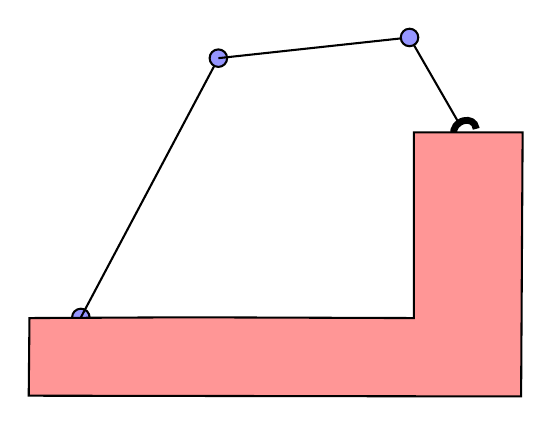
\begin{tikzpicture}[x=0.55pt,y=0.55pt,yscale=-1,xscale=1]
%uncomment if require: \path (0,300); %set diagram left start at 0, and has height of 300

%Shape: Circle [id:dp2680036705913309] 
\draw  [fill=myblue  ,fill opacity=1 ] (144.5,190.35) .. controls (144.5,187.17) and (147.07,184.6) .. (150.25,184.6) .. controls (153.43,184.6) and (156,187.17) .. (156,190.35) .. controls (156,193.53) and (153.43,196.1) .. (150.25,196.1) .. controls (147.07,196.1) and (144.5,193.53) .. (144.5,190.35) -- cycle ;
%Straight Lines [id:da511009501867824] 
\draw    (150.25,190.35) -- (240.6,20) ;
%Shape: Circle [id:dp33456176340238253] 
\draw  [fill=myblue  ,fill opacity=1 ] (234.85,20) .. controls (234.85,16.82) and (237.42,14.25) .. (240.6,14.25) .. controls (243.78,14.25) and (246.35,16.82) .. (246.35,20) .. controls (246.35,23.18) and (243.78,25.75) .. (240.6,25.75) .. controls (237.42,25.75) and (234.85,23.18) .. (234.85,20) -- cycle ;
%Straight Lines [id:da8106680503102979] 
\draw    (240.6,20) -- (366.2,6.4) ;
%Straight Lines [id:da7152287278059997] 
\draw    (399.4,64) -- (366.2,6.4) ;
%Shape: Circle [id:dp1080265764134869] 
\draw  [fill=myblue  ,fill opacity=1 ] (360.45,6.4) .. controls (360.45,3.22) and (363.02,0.65) .. (366.2,0.65) .. controls (369.38,0.65) and (371.95,3.22) .. (371.95,6.4) .. controls (371.95,9.58) and (369.38,12.15) .. (366.2,12.15) .. controls (363.02,12.15) and (360.45,9.58) .. (360.45,6.4) -- cycle ;
%Shape: Block Arc [id:dp8677516838116468] 
\draw  [fill={rgb, 255:red, 0; green, 0; blue, 0 }  ,fill opacity=1 ] (397.16,75.17) .. controls (396.21,74.66) and (395.39,73.93) .. (394.76,73.02) .. controls (392.25,69.38) and (393.66,64.05) .. (397.92,61.11) .. controls (402.18,58.16) and (407.67,58.73) .. (410.18,62.36) .. controls (410.82,63.28) and (411.2,64.3) .. (411.35,65.37) -- (408.23,66.19) .. controls (408.19,65.47) and (407.96,64.78) .. (407.55,64.18) .. controls (406.04,62) and (402.55,61.8) .. (399.74,63.74) .. controls (396.94,65.68) and (395.88,69.02) .. (397.39,71.2) .. controls (397.8,71.8) and (398.37,72.25) .. (399.02,72.54) -- cycle ;
%Shape: Polygon [id:ds12621320375323086] 
\draw  [fill=mypink  ,fill opacity=1 ] (440.5,68.75) -- (369,68.75) -- (369,190.75) -- (219.5,190.25) -- (116.5,190.75) -- (116,241.75) -- (439.5,242.25) -- cycle ;




\end{tikzpicture}

    %\caption{Caption}
    %\label{fig:my_label}
\end{figure}

\end{flushleft}
\end{frame}



\begin{frame}
\centerline{Lecture slides are available via Moodle.}
\bigskip
\centerline{You can help improve these slides at:}
\centerline{\href{https://github.com/SergeiSa/Contact-Aware-Control-Slides-Fall-2020}{github.com/SergeiSa/Contact-Aware-Control-Slides-Fall-2020}}
\bigskip
\centerline{Check Moodle for additional links, videos, textbook suggestions.}
\end{frame}

\end{document}
